	\documentclass{beamer}
	\usepackage[utf8]{inputenc}
	\usepackage[russian]{babel}
    %\usepackage{graphicx} 
    \usepackage{booktabs} 
    \usepackage{beamerthemesplit}
    \setbeamertemplate{footline}[frame number]
    \usepackage{color} %% это для отображения цвета в коде
	\usepackage{listings} 
	\usepackage{graphicx}
	\usepackage{pdflscape,multicol,blindtext}
	\usepackage{amsmath}
	\usepackage{tikz}
	\usepackage{adjustbox}
	\usepackage{listings}
	\usetikzlibrary{}
    \usetheme{PaloAlto}
	\usecolortheme{rose}
	\title[Презентация]{Инструменты для оформления научных статей и презентаций на примере \LaTeX'}
	\institute{КемГУ}
	\author{Дмитрий Басалаев \and Буданцев Артём \and Болковая Полина}
	\date{28.05.2021}
	
\begin{document}
\newlength\someheight
\setlength\someheight{2cm}



\begin{frame}{Титульный слайд}
\maketitle
\end{frame}

\section{Общие цели и задачи}
\begin{frame}{Общие цели и задачи}
\textbf{Цель:} Составить презентацию и отчет о проделанной работе при помощи LateX, задействовав как можно больше его возможностей.
\end{frame}

\section{План график}
\begin{frame}{План график}
\begin{tabular}{| l| p{6.7cm}|}
\hline {\bfseries \large Даты} & {\bfseries \large Действия}\\ \hline
03.02.21-11.03.21. & Изучение базы, установка необходимого софта,подготовка документации\\ \hline
12.03.21-26.03.21 & Изучение интерфейса в \TeX maker, набор простых текстов, спецсимволы \\ \hline
27.03.21-15.04.21 & Ввод математических формул, ввод матриц, спецсимволы  \\ \hline
16.04.21-28.04.21 & Работа с изображениями и встроенной графикой, построение графиков \\ \hline 
29.04.21-14.05.21 & Работа с ссылками,разметка страницы, различные окружения, работа с графикой и презентациями \\ \hline
15.05.21- & Разработка финального продукта, подготовка отчета. \\ \hline
\end{tabular}

\end{frame}

\begin{frame}{Используемые программные средства}
\begin{figure}[h]
\begin{tabular}{cc}

\includegraphics[width=5cm,height=2cm]{texlive}
&

\includegraphics[width=4cm,height=4cm]{texmaker}
\end{tabular}
\end{figure}



\end{frame}

\begin{frame}{27.03.21-15.04.21}
\subsection{27.03.21-15.04.21}
Итак, мы приступили к вводу математических выражений и формул. Желая начать с чего-то простого мы решили преписать школьную таблицу производных и интегралов.
\begin{figure}[h!]
\setlength{\fboxsep}{0pt}%
\setlength{\fboxrule}{1pt}%ширина рамки
\fbox{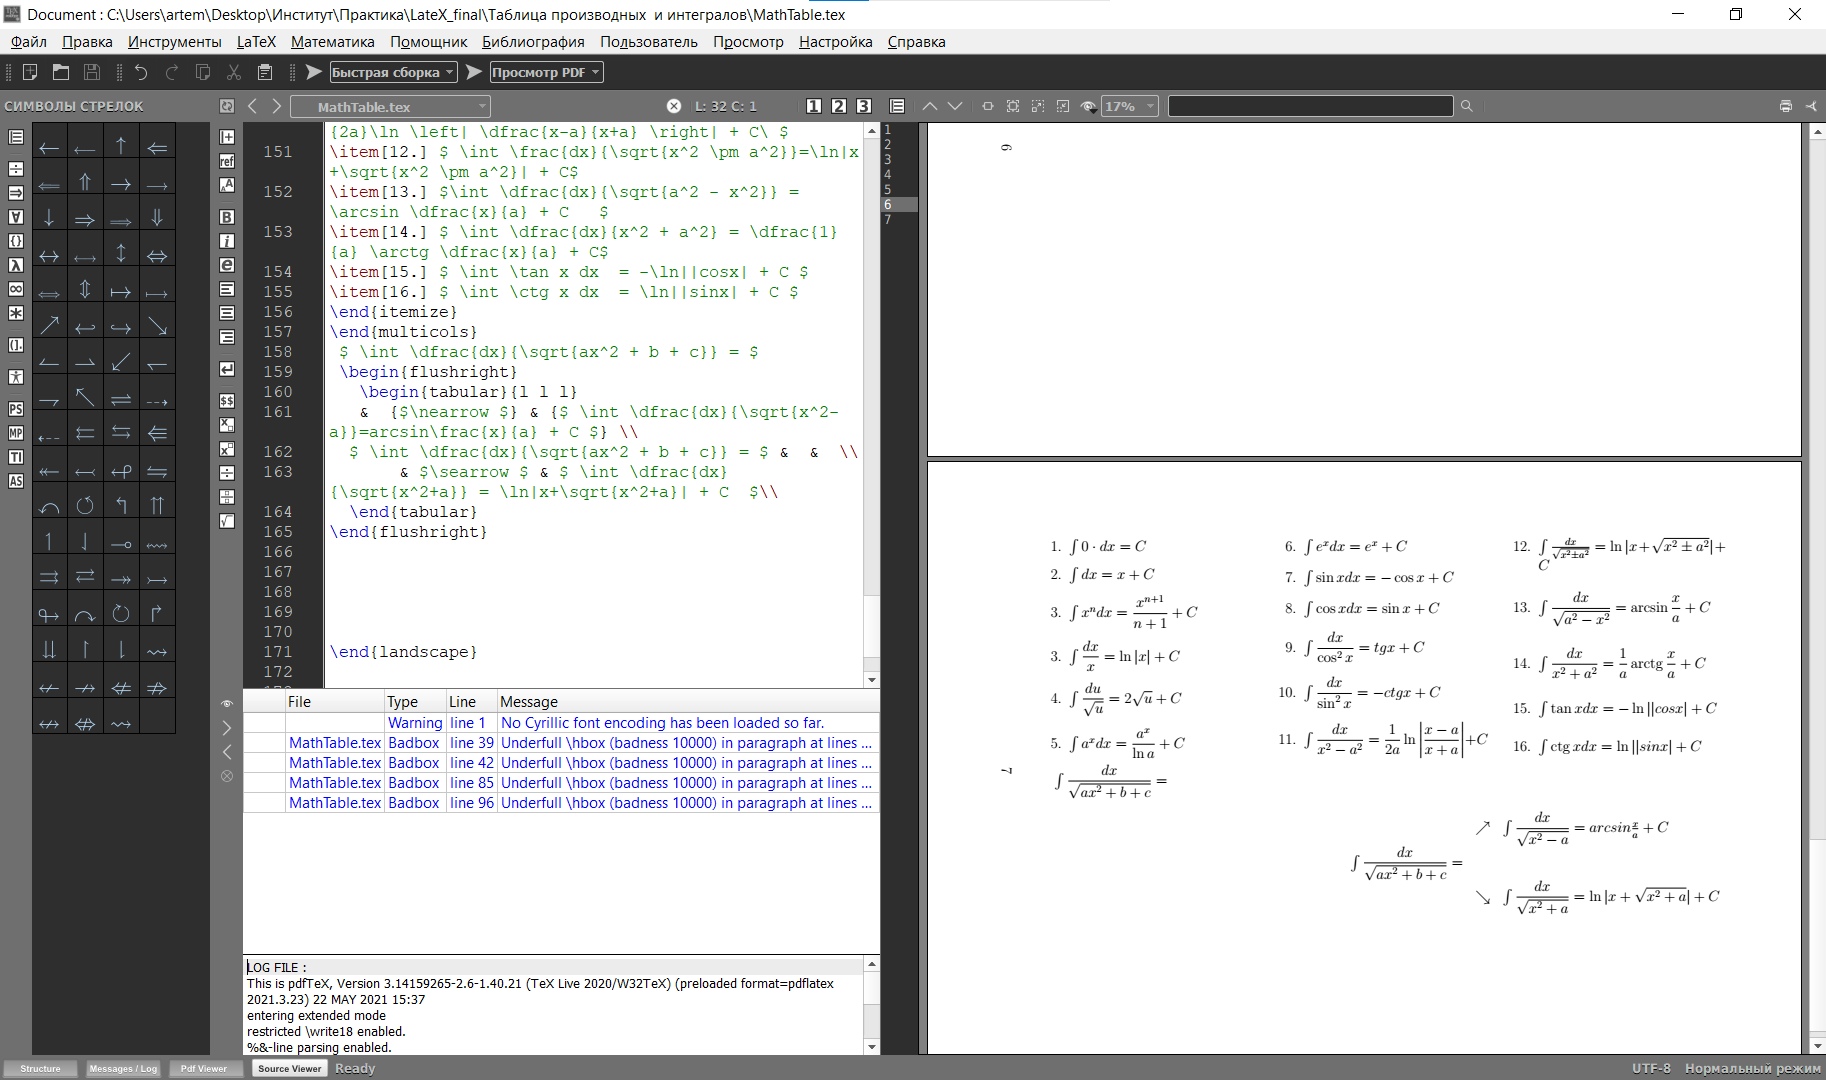
\includegraphics[width=10cm,height=6cm]{Example(1)}}%
\caption{Уже на этом этапе можно понять наскольно в \LaTeX \  проще и быстрее вводить математематические формулы}
\label{fig:image}
\end{figure}
\end{frame}

\begin{frame}

Итак, быстро убедившись что ввод сложных математических формул не представляет трудностей мы приступили к вводу матриц и других крупных объектов.
\begin{figure}[h!]
\setlength{\fboxsep}{0pt}%
\setlength{\fboxrule}{1pt}%ширина рамки
\fbox{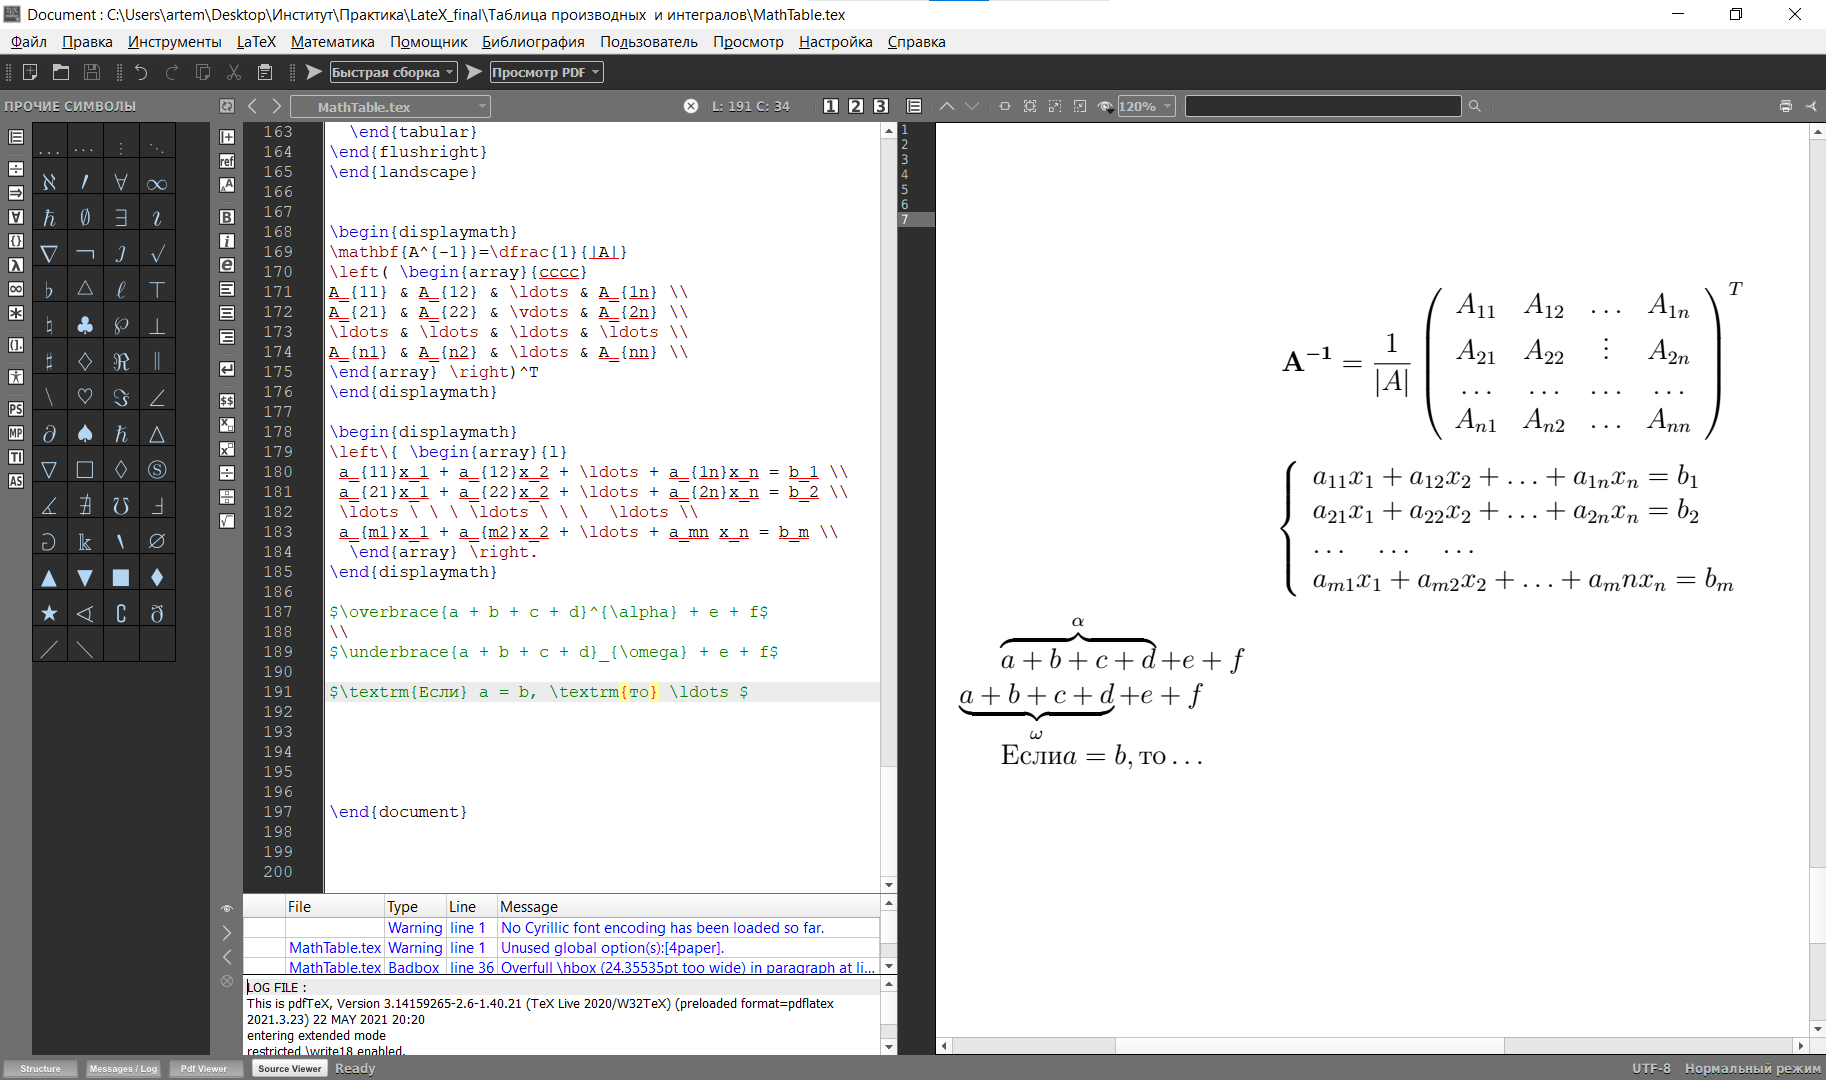
\includegraphics[width=6cm,height=3cm]{Matrrix(1)}}%
\caption{"Крупные" математические объекты}
\end{figure}

\end{frame}

\begin{frame}

Что же касается спец символов, в \LaTeX 'e их огромное количество но раз уж речь идет о математике, то давайте попробуем собрать определение последовательности на языке " $\varepsilon \ \Delta $'
$$\lim_{x \rightarrow x_0}f(x) = A \  \Leftrightarrow \   \forall \ \varepsilon > 0, \ \exists \delta \ >0, |\forall x \ 0<|x-x_0|<\delta \ \Rightarrow |f(x) - A|< \varepsilon   $$


$$\lim_{x \rightarrow 0}\frac{\sin x}{x} = 1  $$

$$\lim_{x \rightarrow \infty} \left( 1 + \frac{1}{x} \right)^x = e  $$

%$\lim_{x \rightarrow 0} \dfrac{sinx}{x} = 1$

\end{frame}

\begin{frame}
\begin{multicols}{3}
    \begin{itemize}
\item[1.] $ c' = 0 \  (c = const)  $
\item[2.] $ (x^n)' = nx^{n-1} $
\item[3.] $ (\sqrt{x})' = \dfrac{1}{2\sqrt{x}} $
\item[4.] $ (a^x)' = a^x\cdot  \ln{a} $
\item[5.] $ (e^x)' = e^x $
\item[6.] $ (\log_{a} x)' = \frac{1}{x\ln a} $
\item[7.] $ (\ln x)' = \frac{1}{x}  $ 
\item[8.] $(\sin \  x)' = \cos \ x  $ 
\item[9.] $(\cos \  x) = - \sin \ x  $ 
\item[10.] $ (\tan \ x)' = \dfrac{1}{\cos ^2 x}  $
\item[11.] $(\ctg)' = -\dfrac{1}{\sin^2 x}  $
\item[12.] $ (\arcsin \ x)' = \dfrac{1}{\sqrt{1 - x^2}}  $ 
\item[13.] $ (\arccos \ x)' = -\dfrac{1}{\sqrt{1 - x^2}}  $ 
\item[14.] $ (\arctan \ x)' = \dfrac{1}{1 + x^2} $
\item[15.] $ (arcctg  \ x)' = -\dfrac{1}{1 + x^2} $
\item[16.] $ (\sinh x)' = \cosh \ x $
\item[17.] $ (\cosh x)' = \sinh \ x $
\item[18.] $ (\tanh x)' = \dfrac{1}{\cosh^2 x}
 $
 \item[19.] $ (cth \  x)' = -\dfrac{1}{\sinh^2 x}
 $
\end{itemize}
\end{multicols}
\end{frame}

\begin{frame}[fragile]{Исходный код}
\begin{adjustbox}{width=15cm,height=3.5cm,keepaspectratio}
 \begin{lstlisting}[language=Tex]

\item[1.] $ c' = 0 \  (c = const)  $
\item[2.] $ (x^n)' = nx^{n-1} $
\item[3.] $ (\sqrt{x})' = \dfrac{1}{2\sqrt{x}} $
\item[4.] $ (a^x)' = a^x\cdot  \ln{a} $
\item[5.] $ (e^x)' = e^x $
\item[6.] $ (\log_{a} x)' = \frac{1}{x\ln a} $
\item[7.] $ (\ln x)' = \frac{1}{x}  $ 
\item[8.] $(\sin \  x)' = \cos \ x  $ 
\item[9.] $(\cos \  x) = - \sin \ x  $ 
\item[10.] $ (\tan \ x)' = \dfrac{1}{\cos ^2 x}  $
\item[11.] $(\ctg)' = -\dfrac{1}{\sin^2 x}  $
\item[12.] $ (\arcsin \ x)' = \dfrac{1}{\sqrt{1 - x^2}}  $ 
\item[13.] $ (\arccos \ x)' = -\dfrac{1}{\sqrt{1 - x^2}}  $ 
\item[14.] $ (\arctan \ x)' = \dfrac{1}{1 + x^2} $
\item[15.] $ (arcctg  \ x)' = -\dfrac{1}{1 + x^2} $
\item[16.] $ (\sinh x)' = \cosh \ x $
\item[17.] $ (\cosh x)' = \sinh \ x $
\item[18.] $ (\tanh x)' = \dfrac{1}{\cosh^2 x}
 $
 \item[19.] $ (cth \  x)' = -\dfrac{1}{\sinh^2 x}
 $
\end{lstlisting}
\end{adjustbox}
\end{frame}

\begin{frame}
\begin{tabular}{l l l} 
   &  {$\nearrow $} & {$ \int \dfrac{dx}{\sqrt{x^2-a}}=arcsin\frac{x}{a} + C $} \\
  $ \int \dfrac{dx}{\sqrt{ax^2 + b + c}} = $ &  &  \\ 
       & $\searrow $ & $ \int \dfrac{dx}{\sqrt{x^2+a}} = \ln|x+\sqrt{x^2+a}| + C  $\\ 
  \end{tabular}

\end{frame}

\begin{frame}[fragile]{Исходный код}
\begin{adjustbox}{scale=0.5}
\begin{large}


 \begin{lstlisting}[language=Tex]
  \begin{tabular}{l l l} 
   &  {$\nearrow $} & {$ \int \dfrac{dx}{\sqrt{x^2-a}}=arcsin\frac{x}{a} + C $} \\
  $ \int \dfrac{dx}{\sqrt{ax^2 + b + c}} = $ &  &  \\ 
       & $\searrow $ & $ \int \dfrac{dx}{\sqrt{x^2+a}} = \ln|x+\sqrt{x^2+a}| + C  $\\ 
  \end{tabular}
\end{lstlisting}
\end{large}
\end{adjustbox}

\end{frame}

\begin{frame}



\begin{displaymath}
\mathbf{A^{-1}}=\dfrac{1}{|A|}
\left( \begin{array}{cccc}
A_{11} & A_{12} & \ldots & A_{1n} \\
A_{21} & A_{22} & \vdots & A_{2n} \\
\ldots & \ldots & \ldots & \ldots \\
A_{n1} & A_{n2} & \ldots & A_{nn} \\
\end{array} \right)^T
\end{displaymath}
\vspace{1cm}
\begin{displaymath}
\left\{ \begin{array}{l}
 a_{11}x_1 + a_{12}x_2 + \ldots + a_{1n}x_n = b_1 \\
 a_{21}x_1 + a_{22}x_2 + \ldots + a_{2n}x_n = b_2 \\
 \ldots \ \ \ \ldots \ \ \  \ldots \\
 a_{m1}x_1 + a_{m2}x_2 + \ldots + a_mn x_n = b_m \\                    
  \end{array} \right.
\end{displaymath}

\end{frame}

\begin{frame}[fragile]{Исходный код}
\begin{adjustbox}{scale=0.7}
\begin{large}


 \begin{lstlisting}[language=Tex]
  \begin{displaymath}
\mathbf{A^{-1}}=\dfrac{1}{|A|}
\left( \begin{array}{cccc}
A_{11} & A_{12} & \ldots & A_{1n} \\
A_{21} & A_{22} & \vdots & A_{2n} \\
\ldots & \ldots & \ldots & \ldots \\
A_{n1} & A_{n2} & \ldots & A_{nn} \\
\end{array} \right)^T
\end{displaymath}
\vspace{1cm}
\begin{displaymath}
\left\{ \begin{array}{l}
 a_{11}x_1 + a_{12}x_2 + \ldots + a_{1n}x_n = b_1 \\
 a_{21}x_1 + a_{22}x_2 + \ldots + a_{2n}x_n = b_2 \\
 \ldots \ \ \ \ldots \ \ \  \ldots \\
 a_{m1}x_1 + a_{m2}x_2 + \ldots + a_mn x_n = b_m \\                    
  \end{array} \right.
\end{displaymath}

\end{lstlisting}
\end{large}
\end{adjustbox}


\end{frame}

\begin{frame}{Использование пакета tikz}


\begin{tikzpicture}
\draw(0,0)--(1,0)--(1.5,-0.5)--(1.5,-2)--(1,-3.5)--(2.5,-4.5)--(3,-4.5)--(3,-4)--(2.5,-4)--(2,-3)--(3,-2.5)--(3.5,-3.5)--(4.5,-4)--(5,-4)--(5,-3.5)--(4.5,-3.5)--(4,-3)--(4,-2.5)--(4.5,-3)--(6.5,-3)--(7,-4.5)--(7.5,-5)--(8,-5)--(8,-4.5)--(7.5,-4.5)--(7.5,-3.5)--(8.5,-4.5)--(9,-4.5)--(9,-4)--(8.5,-4)--(8,-3)--(8.5,-3)--(9,-2.5)--(9,-1)--(8.5,-1.5)--(8,-1.5)--(7.5,-1)--(7.5,-2)--(7,-2)--(5,-1)--(4,-1)--(2.5,-1.5)--(2.5,-0.5)--(1.5,0.5)--(1,0.5)--cycle;
\end{tikzpicture}

\end{frame}

\begin{frame}{Исходный код}
$\backslash$ \textbf{begin\{tikzpicture\} }\\
$\backslash$\textbf{draw(0,0)--(1,0)--(1.5,-0.5)--(1.5,-2)--}\\
\textbf{(1,-3.5)--(2.5,-4.5)--(3,-4.5)}\\
\textbf{--(3,-4)--(2.5,-4)--(2,-3)}\\
\textbf{--(3,-2.5)--(3.5,-3.5)--(4.5,-4)}\\
\textbf{--(5,-4)--(5,-3.5)--(4.5,-3.5)}\\
\textbf{--(4,-3)--(4,-2.5)--(4.5,-3)}\\
\textbf{--(6.5,-3)--(7,-4.5)--(7.5,-5)--}\\
\textbf{(8,-5)--(8,-4.5)--(7.5,-4.5)}\\
\textbf{--(7.5,-3.5)--(8.5,-4.5)--(9,-4.5)}\\
\textbf{--(9,-4)--(8.5,-4)--(8,-3)--(8.5,-3)}\\
\textbf{--(9,-2.5)--(9,-1)--(8.5,-1.5)}\\
\textbf{--(8,-1.5)--(7.5,-1)--(7.5,-2)}\\
\textbf{--(7,-2)--(5,-1)--(4,-1)--(2.5,-1.5)}\\
\textbf{--(2.5,-0.5)--(1.5,0.5)--(1,0.5)--cycle;}\\
$\backslash$\textbf{ end \{ tikzpicture \}}\\
\end{frame}

\begin{frame}

\textbf{Добавление подписей к прямым и углам}\

\begin{tikzpicture}[scale=1.75]
\fill[left color=magenta, right color=yellow]
(0,0) -- node[below=3pt] {$a$} (4,0) --
node[right=5pt] {$b$} (4,3) --
cycle node[midway,above,sloped] {$c=\sqrt{a^2+b^2}$};
\node[below left] at (0,0) {\color{blue}$B$};
\node[below right] at (4,0) {\color{blue}$C$};
\node[above right] at (4,3) {\color{blue}$A$};
\end{tikzpicture}


\end{frame}

\begin{frame}[fragile]{Исходный код}
\begin{adjustbox}{scale=0.8}
\begin{large}


 \begin{lstlisting}[language=Tex]
  \begin{tikzpicture}[scale=1.75]
\fill[left color=magenta, right color=yellow]
(0,0) -- node[below=3pt] {$a$} (4,0) --
node[right=5pt] {$b$} (4,3) --
cycle node[midway,above,sloped] {$c=\sqrt{a^2+b^2}$};
\node[below left] at (0,0) {\color{blue}$B$};
\node[below right] at (4,0) {\color{blue}$C$};
\node[above right] at (4,3) {\color{blue}$A$};
\end{tikzpicture}

\end{lstlisting}
\end{large}
\end{adjustbox}
\end{frame}


















\begin{frame} {Текст}
       \begin{enumerate}
       
       
       \item Текст - ещё текст
       \item Текст - ещё текст
       \item Текст - ещё текст
       \end{enumerate}
       
       
       
       
\end{frame}



\section{Блоки}
\subsection{Текст}
\begin{frame}
	\frametitle{\insertsection}
	\framesubtitle{\insertsubsection}
	\begin{block}<-1>{Первый блок}
		Текст
	\end{block}
	\begin{block}{Второй блок}
		Текст
	\end{block}
	
\end{frame}










\begin{frame}{Конец}
\centering
\huge
Спасибо за внимание!

\end{frame}





\end{document}



